\documentclass{article}
\usepackage{float}
\usepackage{graphicx}
\usepackage[margin=1in]{geometry}
\usepackage{amsmath}
\DeclareMathOperator*{\argmax}{\arg\!\max}
\DeclareMathOperator*{\argmin}{\arg\!\min}

\usepackage{relsize}
\newcounter{lecnum}
\usepackage{placeins}

\newcommand{\lecture}[5]{
   \newpage
   \setcounter{lecnum}{#1}
   \noindent

   \begin{center}
   \framebox{
      \vbox{\vspace{2mm}
    \hbox to 16cm { {\bf CS768 Learning with Graphs
                        \hfill 2020-21 Sem I} }
       \vspace{4mm}
       \hbox to 16cm { {\Large \hfill Lecture #1: #2  \hfill} }
       \vspace{2mm}
       \hbox to 16cm { {\it Scribe: #4 \hfill Updated By: #5  \hfill  Lecturer: #3} }
      \vspace{2mm}}
   }
   \end{center}
   \vspace*{4mm}
}

\newtheorem{theorem}{Theorem}[lecnum]
\newtheorem{lemma}[theorem]{Lemma}
\newtheorem{proposition}[theorem]{Proposition}
\newtheorem{claim}[theorem]{Claim}
\newtheorem{corollary}[theorem]{Corollary}
\newtheorem{definition}[theorem]{Definition}
\newtheorem{que}{Que}




\begin{document}

%\lecture{**LECTURE-NUMBER**}{**DATE**}{**LECTURER**}{**SCRIBE**}
\lecture{7}{September 13}{Abir De}{Kaveri Kale}{Niraj Mahajan}


\section{Supervised Methods For Link Prediction}
\subsection{Outline}
In this lecture we will see how to design and train a supervised link predictor. Following are the steps in designing a supervised link predictor:
\begin{itemize}
  \item Model formulation
  \item Feature construction
  \item Loss function selection
  \item Training
\end{itemize}
\subsection{Train Test Data Split}
Consider a social network $G = (V, E)$ in which each edge
$e = (u, v) \in E$ represents an interaction between u and
v at a particular time t. We split them into training and testing set as follows: 
\begin{enumerate}
    \item Begin with a percentage $\eta$ for the test-train split.
    \item For every node u $\in$ V, assign $\eta$\% edges connected to u to the test set and the remaining to the train set.
    \item Repeat step 2 for all the non edges at u.
    \item Note that the final percentage of test to train edges or non edges may not match $\eta$. This initial $\eta$ will have to be tuned to finally obtain a certain $\eta'$
\end{enumerate}
\subsection{Supervised Predictor using Heuristic based scores}
\noindent In the previous lecture we saw link prediction heuristics like Adamic Adar, Preferential Attachment, Common Neighbor which produce the score for an edge between nodes (u, v), \\
\begin{eqnarray*}
s_{AA}(u, v) = AA(u, v) \\
s_{PA}(u, v) = PA(u, v) \\
s_{CN}(u, v) = CN(u, v)
\end{eqnarray*}
In unsupervised methods, this score is used to rank node pairs in the network. The top ranked pairs are predicted to be connected.\\

We first look at supervised methods, which take the scores from the above mentioned heuristics as features vectors, and perform a classification task.
\begin{equation} \
\begin{split}
s_W & = b + W_{AA} AA(u, v) + W_{CN} CN(u, v) + W_{PA} PA(u, v) \\
 & = \textbf{W}^T \begin{bmatrix}
1 \\
AA(u, v)\\
CN(u, v)\\
PA(u, v)\\
\end{bmatrix}\
\end{split}
\end{equation}
Henceforth, we refer to AA(u,v) as AA for simplicity (similarly PA, CN) \\
         For each pair (u, v) we can define model,
         \begin{equation} \label{}
\begin{split}
s_w(u, v)  & = \textbf{W}^T \begin{bmatrix}
1\\
AA\\
CN\\
PA\\
\end{bmatrix}_{(u, v)}\
\end{split}
\end{equation}
Here $s_W(u, v)$ is parameterized by W and it is stack value of,
   \begin{equation} \label{}
\begin{split}
 \textbf{W}^T =  \begin{bmatrix}
b \\
W_{AA}\\
W_{CN}\\
W_{PA}\\
\end{bmatrix}\
\end{split}
\end{equation} 
\hspace{4in} here b is the bias\\
\subsection{Feature vectors from nodes}
We can also define feature vectors of different nodes which can be the inherent properties of each node.
Consider a graph which has two nodes u, v
We define features for each node.
\begin{equation}
\mathbf{f_u}  :- 
\begin{bmatrix}
f_{u1} \\
f_{u2} \\
.\\
.\\
.\\
f_{un} \\
\end{bmatrix}  \; \& \;
\mathbf{f_v} :- 
\begin{bmatrix}
f_{v1} \\
f_{v2} \\
.\\
.\\
.\\
f_{vn} \\
\end{bmatrix}
\end{equation}
\\
Here we can formulate the model,
\begin{align} \
similarity(u, v) & = \Omega(\mathbf{f_u} , \mathbf{f_v}) \\
\end{align}
where $\Omega$ is a similarity metric, like cosine similarity or rbf similarity
\begin{align} \
\Omega_{cosine}(X, Y) & = \frac{X.Y}{||X||_2 ||Y||_2} \\
\Omega_{rbf}(X, Y) & = e^{-\alpha(||X-Y||^2)}
\end{align}
Given a training graph $ G_{Training} = (V, E_{Training}) $ we can model $s_W(u, v) $ using both the feature similarities and the LP heuristic scores. Let the new feature vector for nodes (u,v) be $f_{uv}$
\begin{align}
s_w(u,v) & = \textbf{W}^T\mathbf{f_{uv}} \\
s_w(u,v) & = \textbf{W}^T 
\begin{bmatrix}
1\\
\Omega(f_u, f_v) \\
AA(u, v)\\
CN(u, v)\\
PA(u, v)\\
\end{bmatrix}
\end{align}
For more complicated model simply use complex structure or dependency between two nodes using more "expressive" predictors.\\
\begin{align} \
s_\theta(u, v) & =NN_\theta(\mathbf{f_{uv}}) \\
\end{align}
Where NN is a neural network\\
\subsection{Training the Network}
We can implement any supervised approach like Linear Regression, Logistic Regression, etc to train our model. Following is an example of training on an SVM.\\
\begin{align} \
(u, v) \in E \;   s_W(u, v ) &\geq 1 - \zeta_{u, v} \\
(u, v) \notin E  \;  s_W(u, v ) &\leq -1 + \zeta_{u, v}
\end{align}
where $\zeta_{u, v}$ is the slack parameter for the node pair (u,v) \\
The optimisation problem for an SVM is given by,
\begin{align}
W_{opt} &= \argmin_W \left\{\frac{1}{2} \lambda ||W||^2 + \sum_{u,v}|\zeta_{u,v}|\right\} 
\end{align}
\hfill subject to $Y_{(u, v)}  s_W(u, v ) \geq 1 - \zeta_{u, v}$ \\
where Y is indicator of edge(+1) or non-edge(-1). \\
\begin{figure}[H]
    \centering
    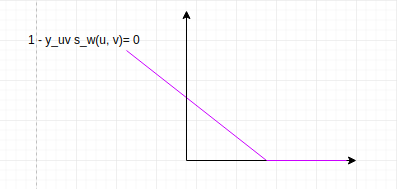
\includegraphics[width=7cm]{hingeloss}
    \caption{Hinge loss}
    \label{fig:hingeloss}
\end{figure}
Here we are trying to construct classifier which will classify edges and non edges.\\
Minimize the loss 
\begin{align} \
\sum_{(u,v) \in {Training}}(1 - Y_{(u, v)}  s_W(u, v ))_+  =
&\sum_{(u,v) \in E_{Training}}(1 -  s_W(u, v ))_+  +
\sum_{(u,v) \in  NE_{G}/NE_{Test-set}}(1 +  s_W(u, v ))_+ 
\end{align}
We can test our trained model on the test set using evaluation metrics like MAP and MRR.\\ \\
\noindent \textbf{Caveat} : Most graphs are sparse, that is,
\begin{align} \
|E| &<< |V| \times |V| \\
|E| &<< |NE|
\end{align}

\noindent Since data is highly imbalanced, learning becomes biased towards the class with the higher cardinality. In our case, the predictor is bound to predict every test set edge/non-edge to be a non-edge \\ In such cases, we add an additional $\Delta$ to make up for this imbalance. \\
Consider $(u, v) \in E_{Training} $ and  $  (u^1, v^1) \notin E_{Training},$ \\
Loss is greater than 0 iff $ s_{W}(u, v)  <  s_{W}(u^1, v^1)  + \Delta \\$ \\
Alternately, we can also scale (divide) the losses due to the edges and the non edges, by the number of edges and non edges in the graph to tackle such imbalanced datasets.
\end{document}